\documentclass[a4paper]{article}

%% Language and font encodings
\usepackage[english]{babel}
\usepackage[utf8x]{inputenc}
\usepackage[T1]{fontenc}
\usepackage{authblk}
\usepackage[usenames, dvipsnames]{color}
\usepackage[table]{xcolor}
%% Sets page size and margins
\usepackage[a4paper,top=2cm,bottom=2.4cm,left = 2 cm, right =2cm]{geometry}

%% Useful packages
\usepackage{amsmath}
\usepackage{amssymb}
\usepackage{graphicx}
\usepackage{mathtools}
%\usepackage{natbib}
\usepackage[colorinlistoftodos]{todonotes}
\usepackage[colorlinks=true, allcolors=blue]{hyperref}

\renewcommand*\familydefault{\sfdefault}
\usepackage[scaled = 0.92]{helvet}


%% define
\definecolor{odd_row}{RGB}{250,250,250}
\definecolor{even_row}{RGB}{217,217,217 }
\definecolor{header}{RGB}{197,197,197 }
\definecolor{footer}{RGB}{57,57,57 }
\font\titlefont=cmr9 at 30pt

%% define header and footer
\usepackage{fancyhdr}
\pagestyle{fancy}
\renewcommand{\headrulewidth}{0.4pt}
\renewcommand{\footrulewidth}{0.4pt}
\lhead{qplum Investment Research}
\rhead{
\includegraphics[width=2cm]{qplum_logo.png}}
\cfoot{\color{footer}\footnotesize
\normalsize\thepage
}


\author[1]{Devendra Bendkhale\thanks{Devendra.Bendkhale@tworoads.co.in}}
\author[1]{Animesh Singh\thanks{Animesh.Singh@tworoads.co.in}}
\author[1]{Gaurav Chakravorty \thanks{gchak@qplum.co}}

\affil[1]{qplum Investment Research}

\title{Relative value trading of interest rate derivatives via deep learning}
\date{}


\begin{document}

\maketitle

\section{Introduction}
This project is mainly about to come up with yield curve from current bond prices and also try to predict future yield curve through ML techniques and then try to find inefficiency among the group of bonds to capture a relative value trade


\section{Yield Curve}
Yield curve is curve showing  several yields or interest rates across different contract lengths (2 month, 2 year, 20 year, etc. ...) for a similar debt contract. It basically depicts the relationship between yield and time to maturity. 
            

\begin{figure}[h!]
\centering
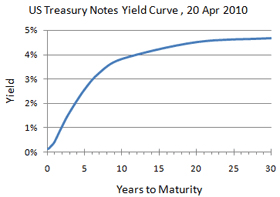
\includegraphics[scale=0.9]{us-treasury-yield.png}
\caption{Yield Curve}
\label{fig:univerise}
\end{figure}
 

\[BondPx
  =\sum_{i=1}^{n-1}\dfrac{C_{i}}{(1+R)^{i}}
\]

Here $C_i$ is the cash flow of the $i^{th}$ year and n is years to maturity to maturity. R is yeild for n year bond. So if we know the coupon rate , then we know all the future cash flows and we can calculate yield from the Market Price of the bond.

 
 \subsection{Spline Fitting}
  Bonds which are traded in the market are quite few . Suppose  we could have only 2,5,10,30 Yr bonds traded in market . So we could have very few points on the yield curve whose exact yield can be calculated from the market price of those bonds. Now , here we are going to use cubic spline fitting between those points to
  get whole yield curve . \\ 
   Spline  is a piecewise polynomial function, made up of individual polynomial sections  or  segments  that  are
   joined  together  at  (user-selected)  points  known as knot
   points.  Cubic spline is a function of  order  three,  and  a piecewise  cubic  polynomial  that  is  twice  differentiable at  each  knot point. At each knot point the slope and curvature of the curve on either side must match. We employ  the  cubic  spline  approach  to  fit  a  smooth curve  to  bond  prices  (yields)  given  by  the discreet maturity bonds traded in market.\\
   Requirements of Cubic Spline are : \\
   \begin{center}
   1. It must equal other cubic polynomial at knot points \\
   2. First derivative should be equal at knot points. \\
   3. Second derivative should be equal at knot points.
  \end{center}
   
   \[ P_i = a_i*x^3 + b_i*x^2 + c_i*x + d_i \]
   
   
   So following are the conditions to be satisfied : 
   \[ P_i(t_i)=y_ \in  [1 , n-1] \] 
   \[ P_i(t_i)=y_i \in  [1 , n-1] \]            
  \[ P_i(t_{i+1})=y_{i+1} \in [2,n]  \]
 \[ P'_i(t_{i+1})=P'_{i+1}(t_{i+1}) \in [1, n-2] \]
 \[  P"_i(t_{i+1})=P"_{i+1}(t_{i+1}) \in [1,n-2] \] \\
 
 
  
  So in total 4n-6 equations 4n-4 unknowns . So this problem has infinite solutions .
  Two extra boundary conditions enforced on these equations would give rise different type of cubic spline fittings having unique solutions. \\
  
  1. Natural Cubic Spline : $P""_0$=0 ,$P""_n$=0 \\
  2. Clamped Cubic Spline : $P'_0$=0 , $P'_0$=0 \\
  
  We could try our intuitions in these boundary conditions or define a metric which could give us desirable fit which we want in yield curve.
  
  
 \section{Prediction of Future Yield Curve}
 Our major aim here is to make a prediction of future yield curve with Prediction Duration of order of hours. One way it could be done by using Trends in the yield curve . We also could use other present yield curves. Also these features could be used with sophisticated ML techniques. \\ \\
 Idea is to come up with general prediction methodology so that we could have better chance to capture inefficiencies in some subset of large product groups. Also , supplementary idea is to trade Bonds with different maturities together . We can also their relative mispricing to be long in one short in another . Group of securities trading together here could used to manipulate PNL variance that suits us to hold positions for very high TTCs. \\
  One Concern is what action to be taken on events . Relative yield curves could be changed due to event information. One option is to getflat before event and resume strategies after event.
  
\section{Obtaining Data}
Currently we are looking out for treasury yield data from some source . Major issue there is that the day which we get is quite not granular .We could find data with daily yield points for Treasury yield curve.

Other option there is to get price data for the trading universe which we want to trade. 
Store price to yield map of the product for range of price values it can approximately take. And then we could get data of any granularity we want . But still Treasury yield data and LIBOR data cannot be obtained of that granularity.
 
 
 
\section{Conclusion}
``I always thought something was fundamentally wrong with the universe'' \citep{adams1995hitchhiker}
 
\iffalse
%Some way to add notes
\fi 

\bibliographystyle{alpha}
\bibliography{refs}
\newpage
\section{Disclosures \label{disclosures} }
All investments carry risk. This material is for informational purposes only. The factual information set forth herein has been obtained or derived from sources believed to be reliable but it is not necessarily all-inclusive and is not guaranteed as to its accuracy and is not to be regarded as a representation or warranty, express or implied, as to the information’s accuracy or completeness, nor should the attached information serve as the basis of any investment decision. Past performance is not indicative of future performance. Please visit our website \url{https://www.qplum.co/privacy-terms#disclaimer} for full disclaimer and terms of use.\\
This document is intended exclusively for the use of the person to whom it has been delivered and it is not to be reproduced or redistributed to any other person.

\end{document}
